\section{MANO Benchmarking Framework} 

\subsection{Introduction}

MANO Benchmarking Framework (MBF) is a result of a small script that was used to run the experiments discussed in the previous sections. 
The idea of MBF is to provide MANO developers with a generic framework for running experiments on MANO. 
MBF mainly provides the following 1) Easy interfacing with MANO instances by using python-mano-wrappers, 2) Ability to run experiments with different service descriptors, 3) Collection of performance metrics in convenient data format and 4) Flexible graphing mechanism of the collected data. 


\subsection{Design}

MBF is designed for ease of use and low barrier to entry for developers. 
We explain the choice of tools that are used in MBF in the following list.

\begin{itemize}
	\item{\textbf{Netdata\footnote{https://github.com/netdata/netdata}}} is the metrics monitoring system for MBF. 
	Netdata captures relevant system metrics and provide powerful APIs to query the recorded data in a suitable format.
	\item{\textbf{Python}} as the choice of scripting language was obvious as the MANOs itself are implemented in python.
	\item{\textbf{python-mano-wrappers}} is used to provide access to REST APIs of MANOs from python.
	\item{\textbf{Docker}} is used to containerize MBF, thus making it easy to distribute and portable.
	\item{\textbf{Matplotlib}} is the graphing library for MBF due to its flexibility and ease of use.
	\item{\textbf{Flask}} as a python server that can be used to provide additional interactions with the experiment runner.

\end{itemize}


\subsection{Parameters and KPIs} 

\subsubsection{Parameters}

MBF has experiment parameters that can be altered. The following paramenters are supported

\begin{itemize}
	\item{\textbf{Descriptors}} NSDs and VNFDs can be changed. a list of NSDs/VNFDs is also supported. When a list of descriptors are provided, the experiment will be run for each of the descriptors.
	\item{\textbf{Number of instances}} Total number of instantiation requests to be sent to the MANO.
	\item{\textbf{Number of runs}} number of re-runs of the same experiment to be run. 
	This is performed to measure the variance in results.
	\item{\textbf{Requests per minute (RPM)}} The rate at which the instantiation requests are sent to the MANO
	\item{\textbf{Observation Time}} The observation time after the instantiation requests are sent. 
	This can be used to collect metrics post instantiation to observe how MANO behaves in the monitoring phase.
	\item{\textbf{Inter-experiment Delay}} is the time between experiment runs. 
	This is altered to give enough time for the VIM to terminate and cleanup instances from the previous experiment runs if any.
	\item{\textbf{Skip experiment on error}} if set to true, the current run is skipped due to a failed instance on the VIM.

\end{itemize}

\subsection{Key Performance Indicators}

MBF stores resource utilization metrics during the experiment and generates graphs to visualize the results. 
However, these are only examples and the further possibilities are supported by the framework. 
The metrics are stored as CSV files.

\begin{itemize}
	\item{\textbf{CPU}} Overall system CPU usage is recorded as well as the individual docker micro service CPU usage metrics are stored.
	\item{\textbf{Memory}} Overall system memory usage along with the individual docker micro service memory usage is stored.
	\item{\textbf{System Load}} The 1m, 5m and 15m moving averages of system load values provided by the linux kernel is stored.
	\item{\textbf{Status Tracking}} The status of all instances are stored by polling the VIM every 5 seconds over the experiment lifetime. 
	This enables to track the status change over time.
	\item{\textbf{End-to-end Deployment Time}} is the time elapsed to deploy all the instances on the VIM.
	\item{\textbf{Individual Deployment Time}} is the time taken by each instance for deployment. 
	This is also split into time taken by MANO and VIM.
\end{itemize}

\subsection{Steps for experiment run} 

The steps to run a basic experiment is detailed in this section. 
The following instruction is to run an experiment with 90 instances on OSM using an network service with 1 VNF. 

\begin{enumerate}
	\item Git clone the experiments-branch\footnote{https://github.com/CN-UPB/MANO-Benchmarking-Framework}
	\item Build and start the docker container
	\item Change experiment variables in the relevant scripts for respective MANOs
	\begin{itemize}
		\item \textbf{OSM} -- \textit{run-experiment-osm.py}
		\item \textbf{Sonata (Pishahang)}  -- \textit{run-experiment-sonata.py}
		\item \textbf{Sonata Container Orchestration (Pishahang)} -- \textit{run-experiment-sonata-k8}
	\end{itemize}
	
	\item Run the relevant script from inside the container. 
	The experiment will now run and stores result files in the same directory
	\item Use the result parser from the \texttt{experiments/results/csv-result-parser.py} to parse the results and store it in a format suitable for graphing
	\item Finally use the graph plotter on the parsed files to generate the graphs \texttt{experiments/results/plot-graphs.py}
	
	\end{enumerate}

The commands required to run these are listed in the readme file here, \\ \url{https://github.com/CN-UPB/MANO-Benchmarking-Framework/blob/master/README.md}

\textit{\\\textbf{Note:} This process is being streamlined to reduce some redundant steps and will be released in the next version of MBF.} 

\subsection{Example Use Cases}

In this section we demonstrate a few use cases of MBF. 
The framework facilitated easy experimentation, collection and analysis of metrics in the following cases. 
However, in-depth analysis of what the metrics and graphs mean are out of scope of this document. 



\subsubsection{Comparison of different network services} 

We compared the performance metrics of different NSDs/VNFDs and visualized it. 
For this, we provided 6 different network service descriptors to the experiment runner. 
First 3 NS consisted of a cirros image as a VNF with 1, 3 and 5 VNFs per NSD and the other 3 NS consisted of an ubuntu image as a VNF with 1, 3 and 5 VNFs per NSD.\\

The experiment stores the KPIs listed in the previous section, along with the graphs visualizing the differences. 
This graph is produced for each micro-service showing the resource utilization of each NS under different number of instantiations. 
As an example, the figures \ref{fig:osmlcm-mean-cpu-cases} and \ref{fig:osmro-mean-cpu-cases} show the CPU utilization of the OSM microservice LCM and RO respectively.

\begin{figure}[h]
	\centering
	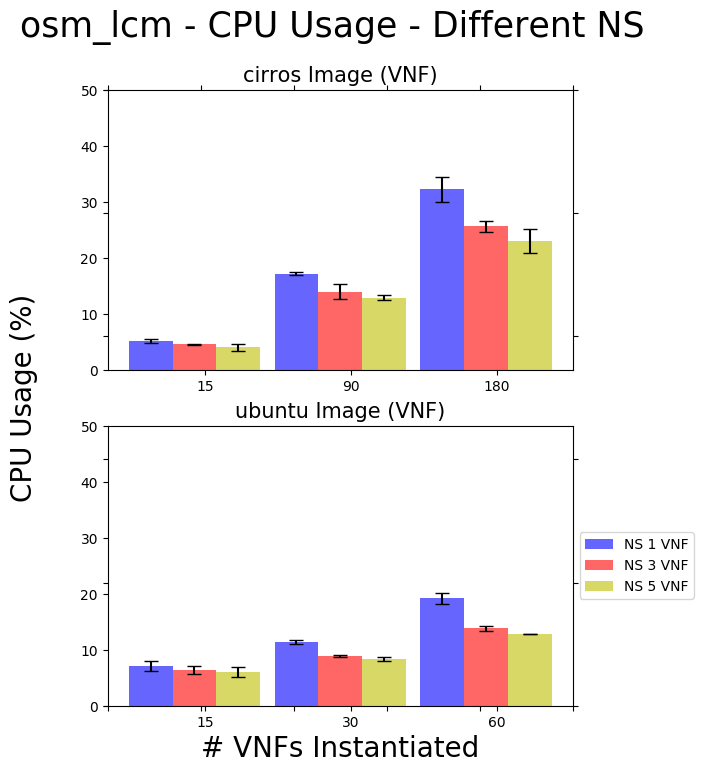
\includegraphics[width=0.6\linewidth]{figures/scalability_graphs/Docker-Grouped-Cases/osm/osm_lcm-Mean-CPU-Cases}
	\caption{CPU usage of OSM microservice LCM}
	\label{fig:osmlcm-mean-cpu-cases}
\end{figure}

\begin{figure}[h]
	\centering
	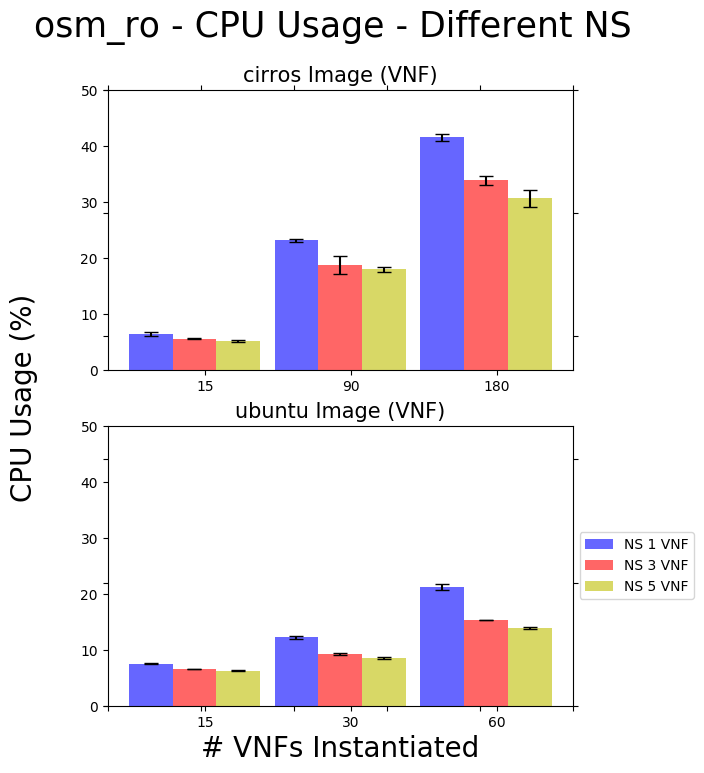
\includegraphics[width=0.6\linewidth]{figures/scalability_graphs/Docker-Grouped-Cases/osm/osm_ro-Mean-CPU-Cases}
	\caption{CPU usage of OSM microservice RO}
	\label{fig:osmro-mean-cpu-cases}
\end{figure}


\subsubsection{Container vs VM Orchestration} 

Pishahang supports container orchestration on kubernetes and OSM supports VM orchestration on OpenStack. 
We compared the performance of orchestrating similar network services on VM and containers. 
In the figure \ref{fig:timecomparison}, the graph on top shows the average time distribution between MANO and VIM for deploying one network service with one VNF. 
The bottom graph in the figure \ref{fig:timecomparison} shows the total time taken to deploy 90 instances of a network with one VNF. 
The time taken to deploy similar VNFs is significantly less for containers, which is expected as containers are light weight compared to a VMs. \\

\textit{Note:} Pishahang support for VM orchestration is not stable, hence, we could not perform similar VM experiments on Pishahang for this comparison.

\begin{figure}[h]
	\centering
	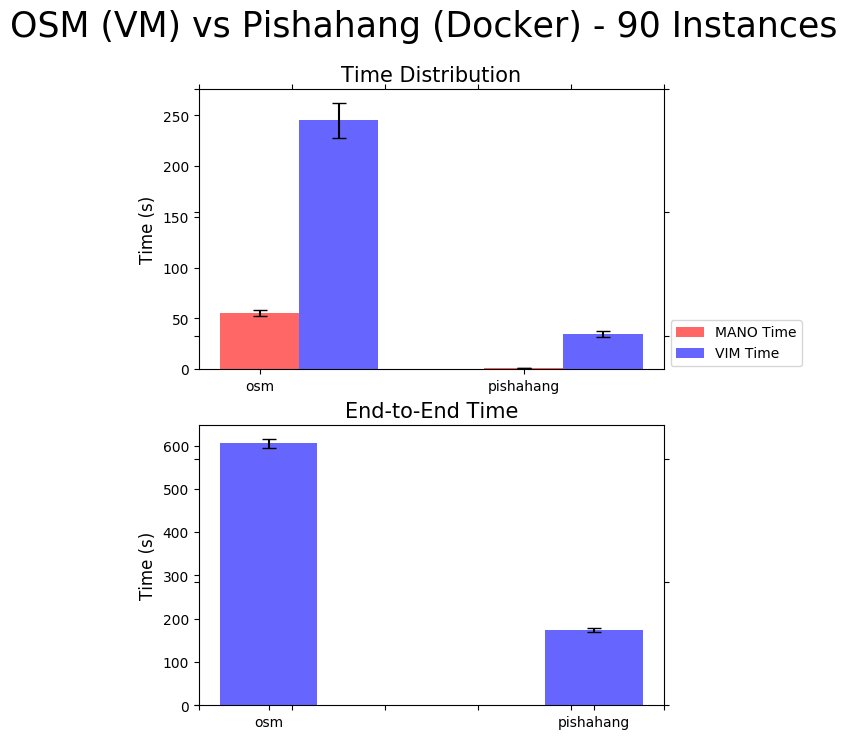
\includegraphics[width=0.7\linewidth]{figures/scalability_graphs/Comparison-VM-Docker/Time_comparison}
	\caption{Time distribution in MANO and VIM}
	\label{fig:timecomparison}
\end{figure}


\begin{figure}[h]
	\centering
	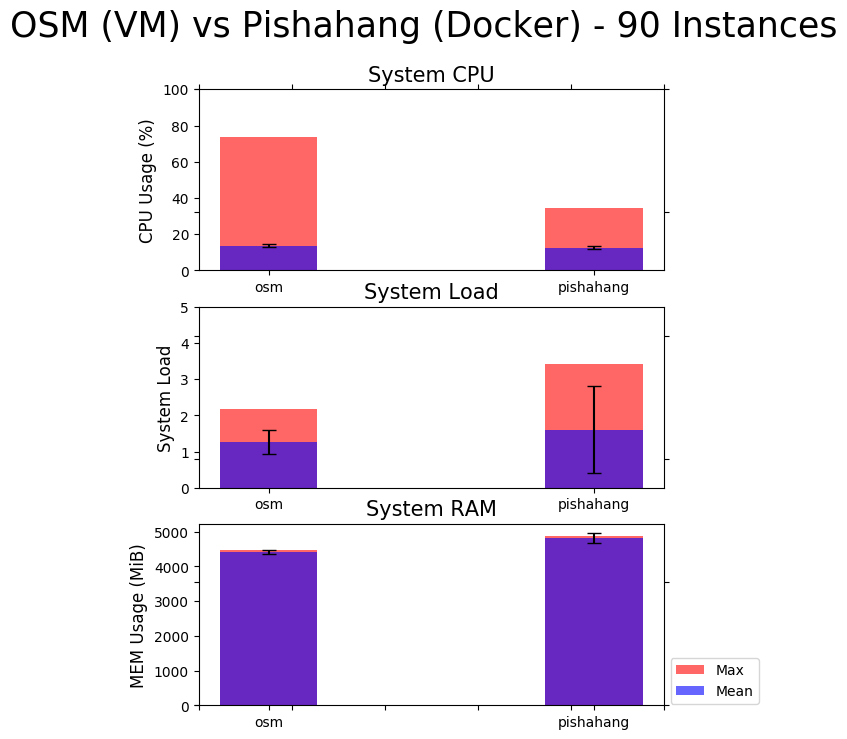
\includegraphics[width=0.7\linewidth]{figures/scalability_graphs/Comparison-VM-Docker/System_metrics_comparison}
	\caption{System resource utilization}
	\label{fig:systemmetricscomparison}
\end{figure}


\subsubsection{Scaling Plugin Evaluation}

\todo[inline]{To be filled along with the scalability plugin docs}

Child MANO lifecycle graph \ref{fig:child-top-3-lifecycle}. 
Parent MANO lifecycle graph \ref{fig:parent-top-3-lifecycle}. 

\begin{figure}[h]
	\centering
	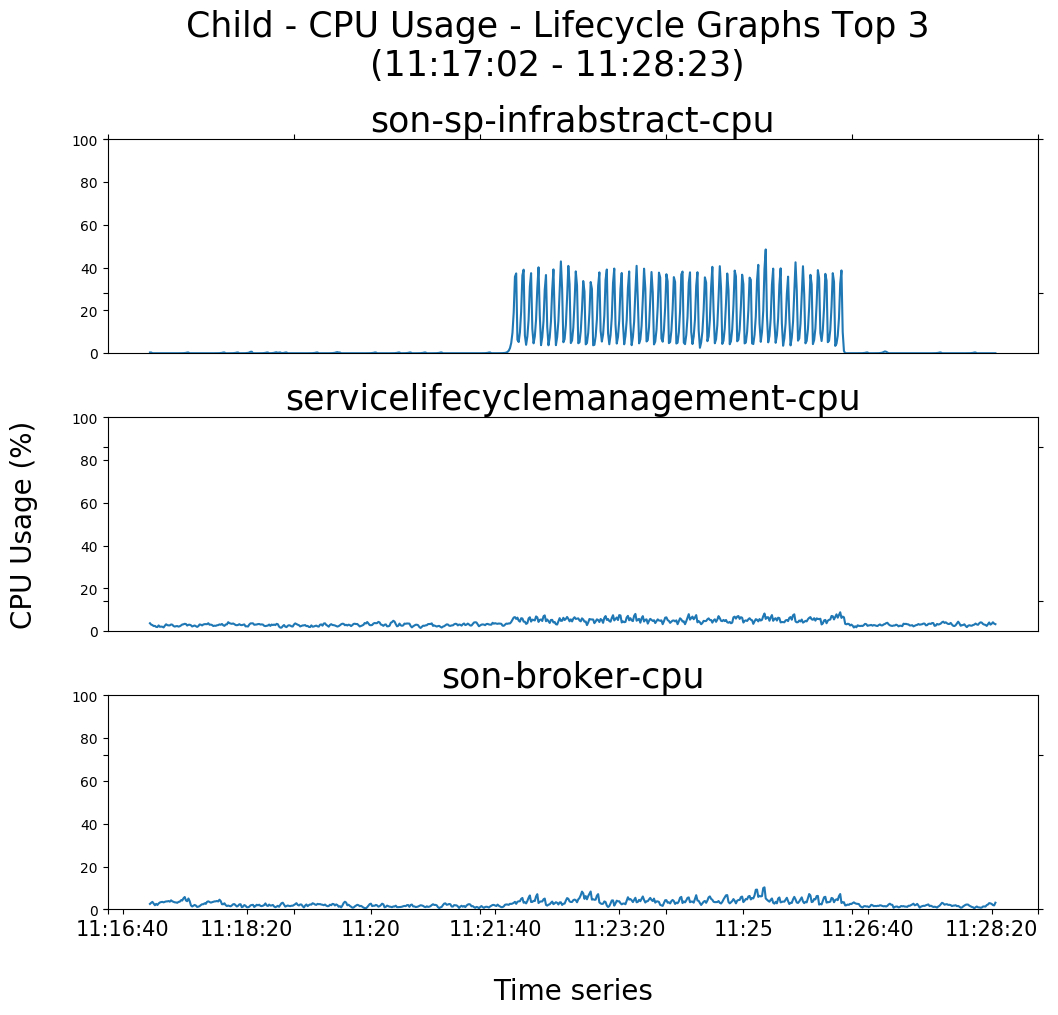
\includegraphics[width=0.7\linewidth]{figures/scalability_graphs/Scalability-Evaluation/Child-TOP-3-Lifecycle}
	\caption{Child scaling}
	\label{fig:child-top-3-lifecycle}
\end{figure}

\begin{figure}[h]
	\centering
	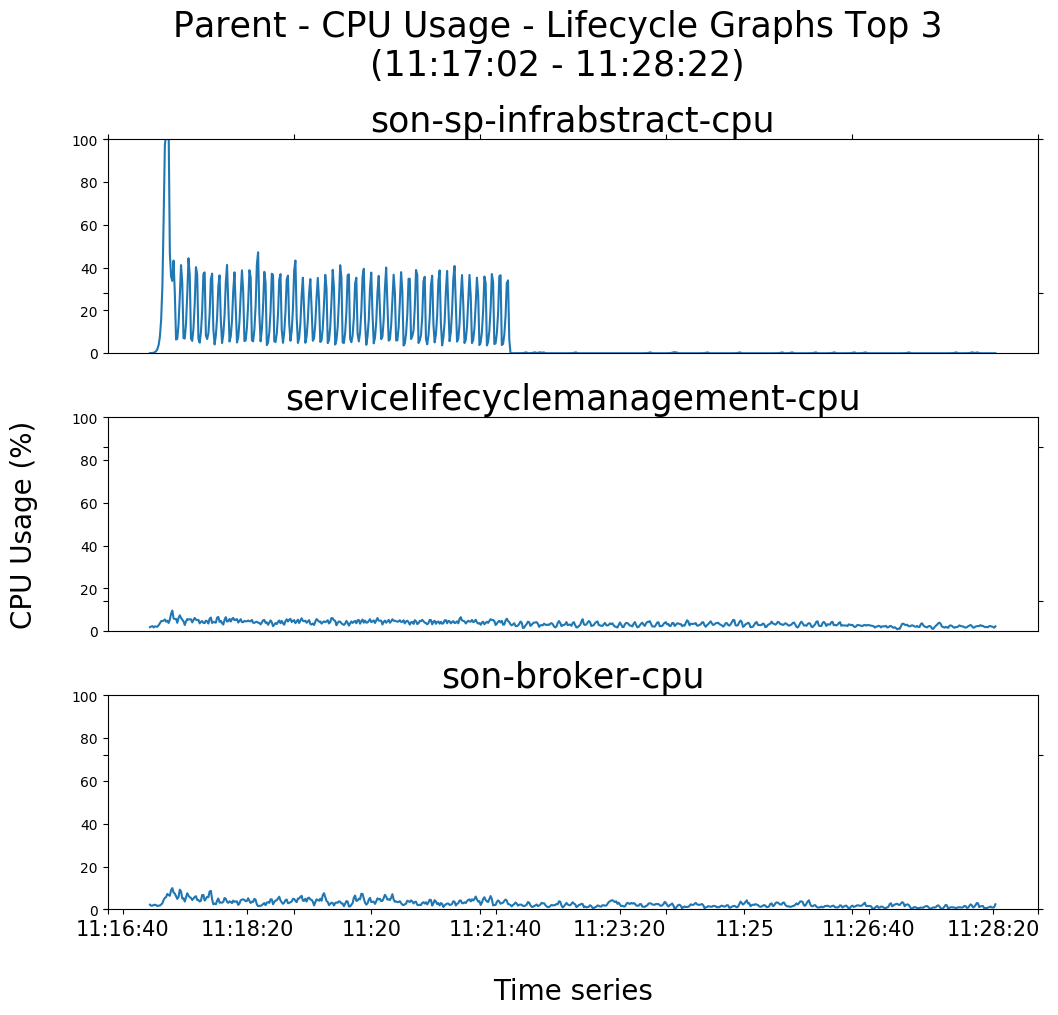
\includegraphics[width=0.7\linewidth]{figures/scalability_graphs/Scalability-Evaluation/Parent-TOP-3-Lifecycle}
	\caption{Parent Scaling}
	\label{fig:parent-top-3-lifecycle}
\end{figure}


\subsection{Future scope}